\documentclass{article}
\usepackage[czech]{babel}
\usepackage{graphicx} % Required for inserting images
\usepackage{float}
\graphicspath{ {./img/} }
\sloppy

\title{LAESA}
\author{Jan Kimr}
\date{16. dubna 2023}

\begin{document}

\maketitle

\section{Popis projektu}

Cílem projektu je vytvoření implementace metrické přístupové metody (MAM) LAESA (Linear Approximating and Eliminating Search Algorithm), což je algoritmus pro indexování $n$-dimenzionálních objektů v metrickém prostoru. Vstupem algoritmu je seznam $n$-dimenzionálních objektů, funkce splňující axiomy metriky a seznam pivotů. Ve vytvořeném indexu je možné rychle řešit rozsahové a kNN dotazy, jejichž výstupem je seznam objektů, které splňují zadaná kritéria.

Ke zrychlení vyhledávání pomocí LAESA dochází – na rozdíl od sekvenčního průchodu – na základě odfiltrování většiny objektů pomocí dolní meze vzdálenosti, aniž by bylo potřeba počítat vzdálenost mezi zadaným bodem a objektem. Zrychlení je tím výraznější, čím je vzdálenostní funkce časově náročnější.

Projekt obsahuje kromě implementace i jednoduché webové rozhraní pro testování metody a obsáhlou experimentální část v Jupyter notebooku. V experimentální části je testována rychlost a počet volání vzdálenostní funkce v závislosti na různých hodnotách parametrů.

\section{Způsob řešení}
\subsection{Výběr pivotů}
Před samotným vytvořením indexu je třeba nejprve vybrat pivoty. Jednoznačně nejlepší přístup pro výběr pivotů není možné určit, jelikož pro různé dotazy mohou být optimální různé volby pivotů. Možnosti výběru pivotů, které implementace podporuje, jsou: náhodný výběr, seznam zadaný uživatelem a shlukovací algoritmus k-means. Algoritmus k-means rozděluje objekty v databázi do shluků, přičemž optimalizuje účelovou funkci (suma druhých mocnin vzdáleností bodů od geometrických středů shluků, do nichž náleží). Jako pivoty jsou použity geometrické středy vzniklých shluků.

Po výběru pivotů je pro každý objekt v databázi a pro všechny pivoty spočítána vzdálenost. Pro $n$ objektů a $k$ pivotů jsou tyto vzdálenosti uloženy v matici (tzv. tabulce pivotů) o $n$ řádcích a $k$ sloupcích.

\subsection{Rozsahový dotaz}

Při zodpovídání rozsahového dotazu je nejprve vypočítána vzdálenost mezi zadaným bodem a všemi pivoty. Vzdálenost mezi zadaným bodem a libovolným objektem v databázi lze zdola odhadnout jako minimum z dolních odhadů vzdáleností při použití jednotlivých pivotů ($lb_{q,o_i} = min \{ d(q, p) - d(p, o_i)\ |\ p \in P \}$). Pokud je dolní mez vzdálenosti větší než zadaný maximální rozsah, je možné tento objekt odfiltrovat a nepočítat pro něj přesnou vzdálenost pomocí vzdálenostní funkce. Pro body, které zbydou po odfiltrování, je vzdálenost vypočítána a finální odpověď tvoří pouze objekty ve vzdálenosti menší, než je maximální rozsah.

\subsection{kNN dotaz}

kNN dotaz také začíná vypočítáním dolní meze vzdálenosti zadaného bodu od objektů v databázi. Objekty jsou následně uspořádány v pořadí rostoucí dolní meze vzdálenosti. Prvních $k$ objektů je přidáno do maximové prioritní fronty, kde je priorita určena skutečnou vzdáleností bodu od objektu. Následně jsou procházeny uspořádané objekty (od indexu $k+1$ dál) a v případě, že skutečná vzdálenost některého z objektů je menší než objektu na začátku fronty (nejvzdálenější objekt), je objekt ze začátku fronty odstraněn a je přidán objekt s menší vzdáleností. Toto prohledávání je možné ukončit, pokud dolní mez vzdálenosti aktuálně testovaného objektu je větší než skutečná vzdálenost nejvzdálenějšího z k vybraných objeků.

\section{Implementace}

Projekt je implementovaný v jazyce Python3. Pro práci s daty je použita knihovna NumPy, pro grafické zobrazení výsledků knihovna matplotlib, pro shlukování pomocí algoritmu k-means knihovna scikit-learn, webové rozhraní je vytvořeno v HTML s pomocí knihovny PyScript. Projekt obsahuje Jupyter notebook s ukázkami použití a experimenty a dále jednoduché webové rozhraní pro testování dotazů. 

Pro spuštění notebooku je třeba mít nainstalovaný Python3, Miniconda a výše uvedené knihovny (pomocí: \textit{conda env update}; \textit{conda activate bivwm}). Jupyter se spouští pomocí příkazu \textit{jupyter notebook}, webové rozhraní se spouští pomocí příkazu \textit{python3 -m http.server}.

\section{Příklad výstupu}

\begin{figure}[H]
    \centering
    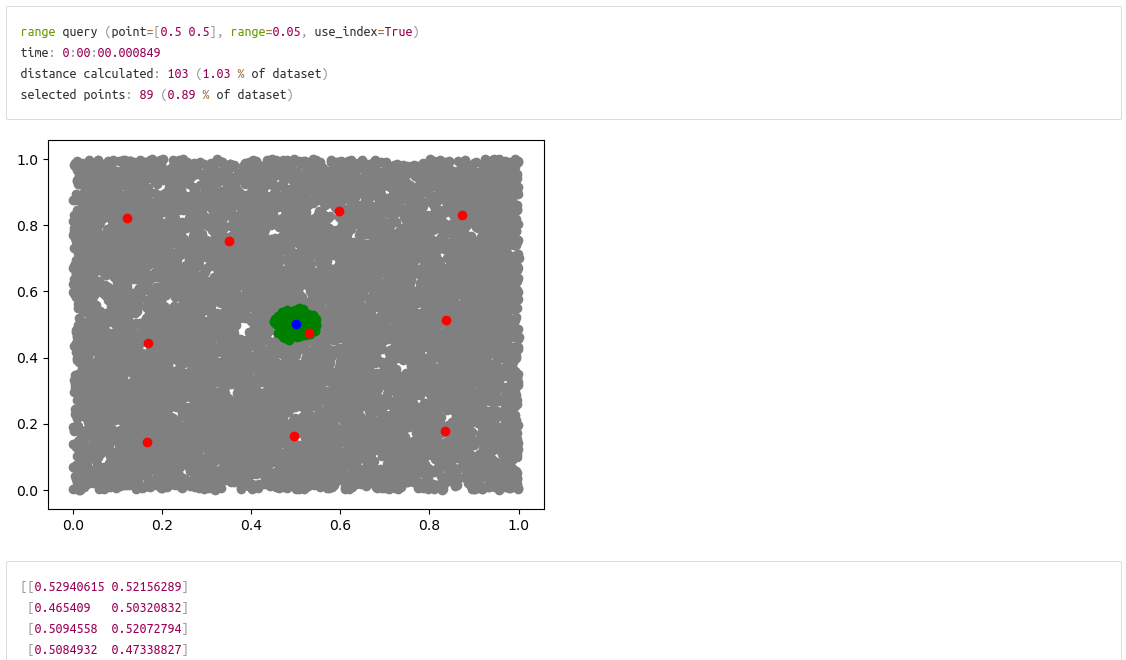
\includegraphics[width=\textwidth]{img/range_2d.png}
    \caption{Ukázka výsledku rozsahového dotazu v 2d indexu v Jupyter notebooku (seznam bodů je pro stručnost zkrácený). Šedá – objekty v databázi, červená – pivoty, zelená – objekty v rozsahu, modrá – zvolený bod.}
\end{figure}

\begin{figure}[H]
    \centering
    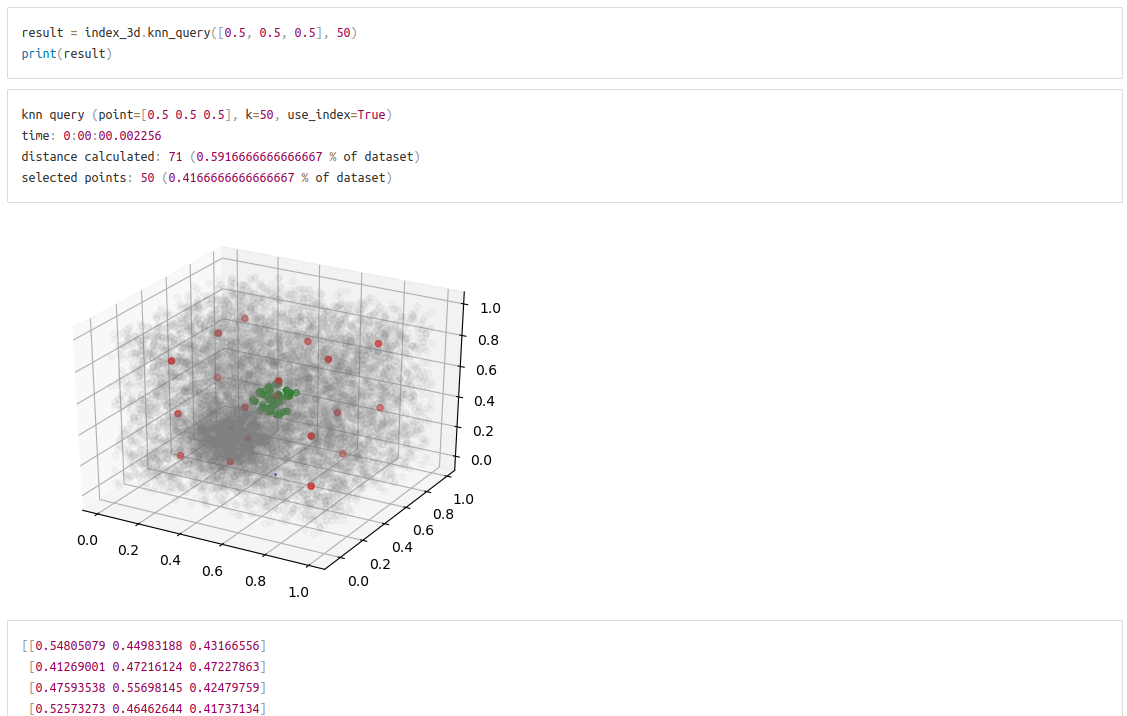
\includegraphics[width=\textwidth]{img/knn_3d.png}
    \caption{Ukázka výsledku kNN dotazu v 3d indexu v Jupyter notebooku (seznam bodů je pro stručnost zkrácený). Šedá – objekty v databázi, červená – pivoty, zelená – objekty v rozsahu, modrá – zvolený bod.}
\end{figure}

\begin{figure}[H]
    \centering
    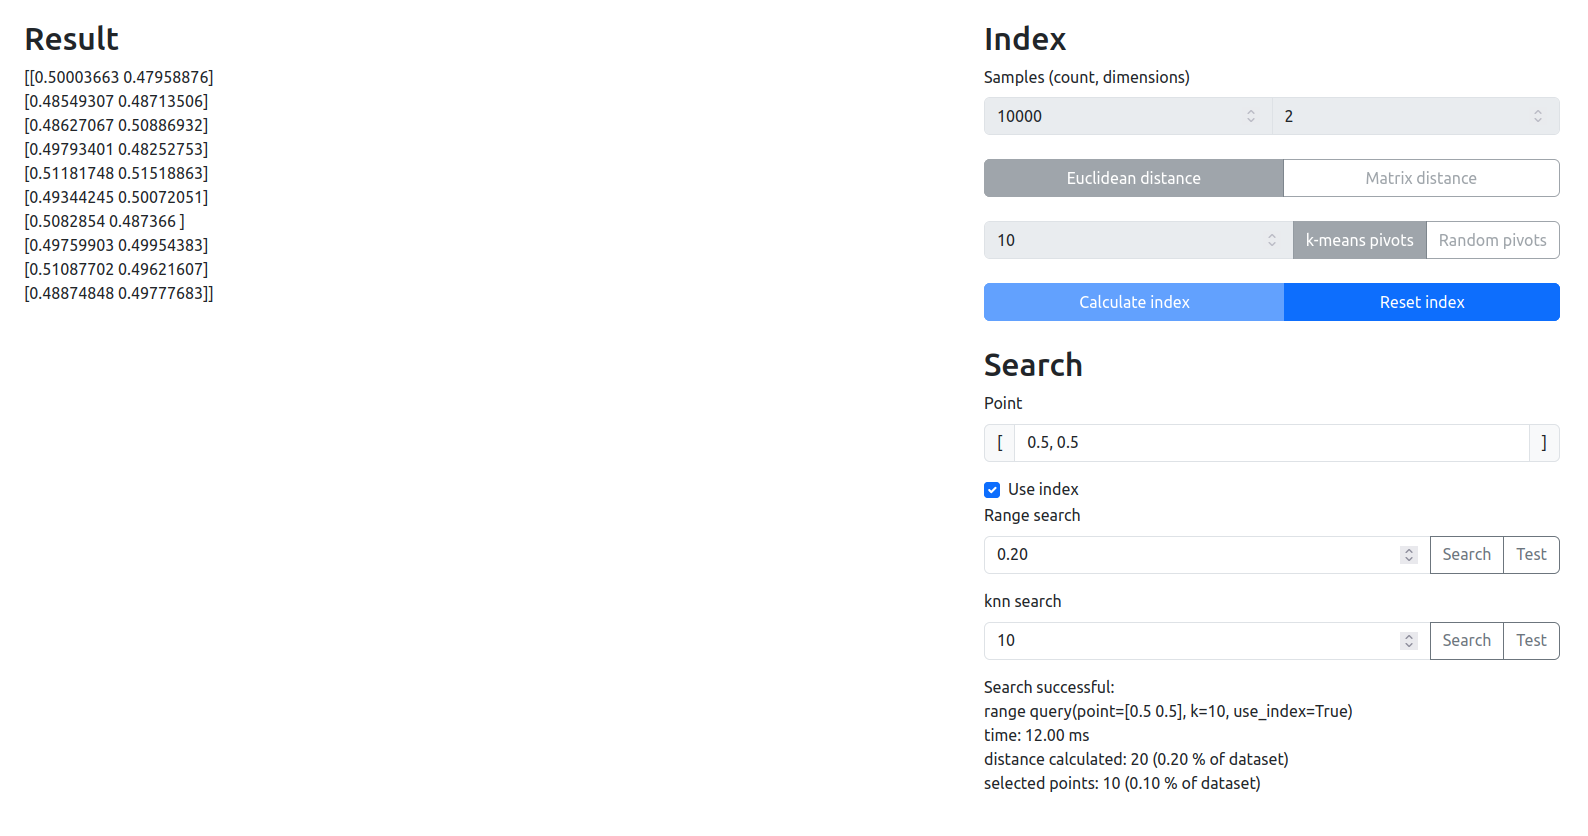
\includegraphics[width=\textwidth]{img/web_gui.png}
    \caption{Ukázka webového rozhraní}
\end{figure}

\section{Experimentální sekce}

U LAESA se nabízí testovat zejména rychlost dotazů, případně počet volání vzdálenostní funkce a vliv různých parametrů na tuto hodnotu, např.: počet pivotů, počet dimenzí, velikost databáze, velikost rozsahu/počtu nejbližších sousedů. Následující testy jsem prováděl na databázi s $10\ 000$ uniformě rozprostřenými 2D objekty s Euklidovskou vzdáleností a s 10 pivoty, které byly určovány pomocí algoritmu k-means (není-li uvedeno jinak). Čas i počet volání vzdálenostní funkce je průměr z dvaceti dotazů v náhodných bodech.

\subsection{Testování optimálního počtu pivotů}
Z pokusů vyplývá, že dobrý počet pivotů je okolo deseti. Tento počet představuje místo zlomu, před nimž dochází k výraznějšímu zlepšení. Naopak větší počet pivotů už obvykle výrazně lepší výsledek nepřináší. U kNN dotazů s $k = 1000$ a $k = 2000$ je zajímavý rozdíl v situaci bez pivotů (sekvenční průchod) a s jedním pivotem. Zhoršení času, ke kterému dochází, si vysvětluji tím, že přidání jednoho pivotu sice sníží počet volání vzdálenostní funkce, ne však o tolik, aby to převážilo výpočetní náročnost přidanou použitím LAESA. V případě, že by časová náročnost vzdálenostní funkce byla výrazně větší, došlo by v situaci s jedním pivotem nejspíše k drobnému zlepšení, jelikož počet volání vzdálenostní funkce je menší v porovnání se situací bez pivotů (sekvenčním průchodem).

\begin{figure}[H]
    \centering
    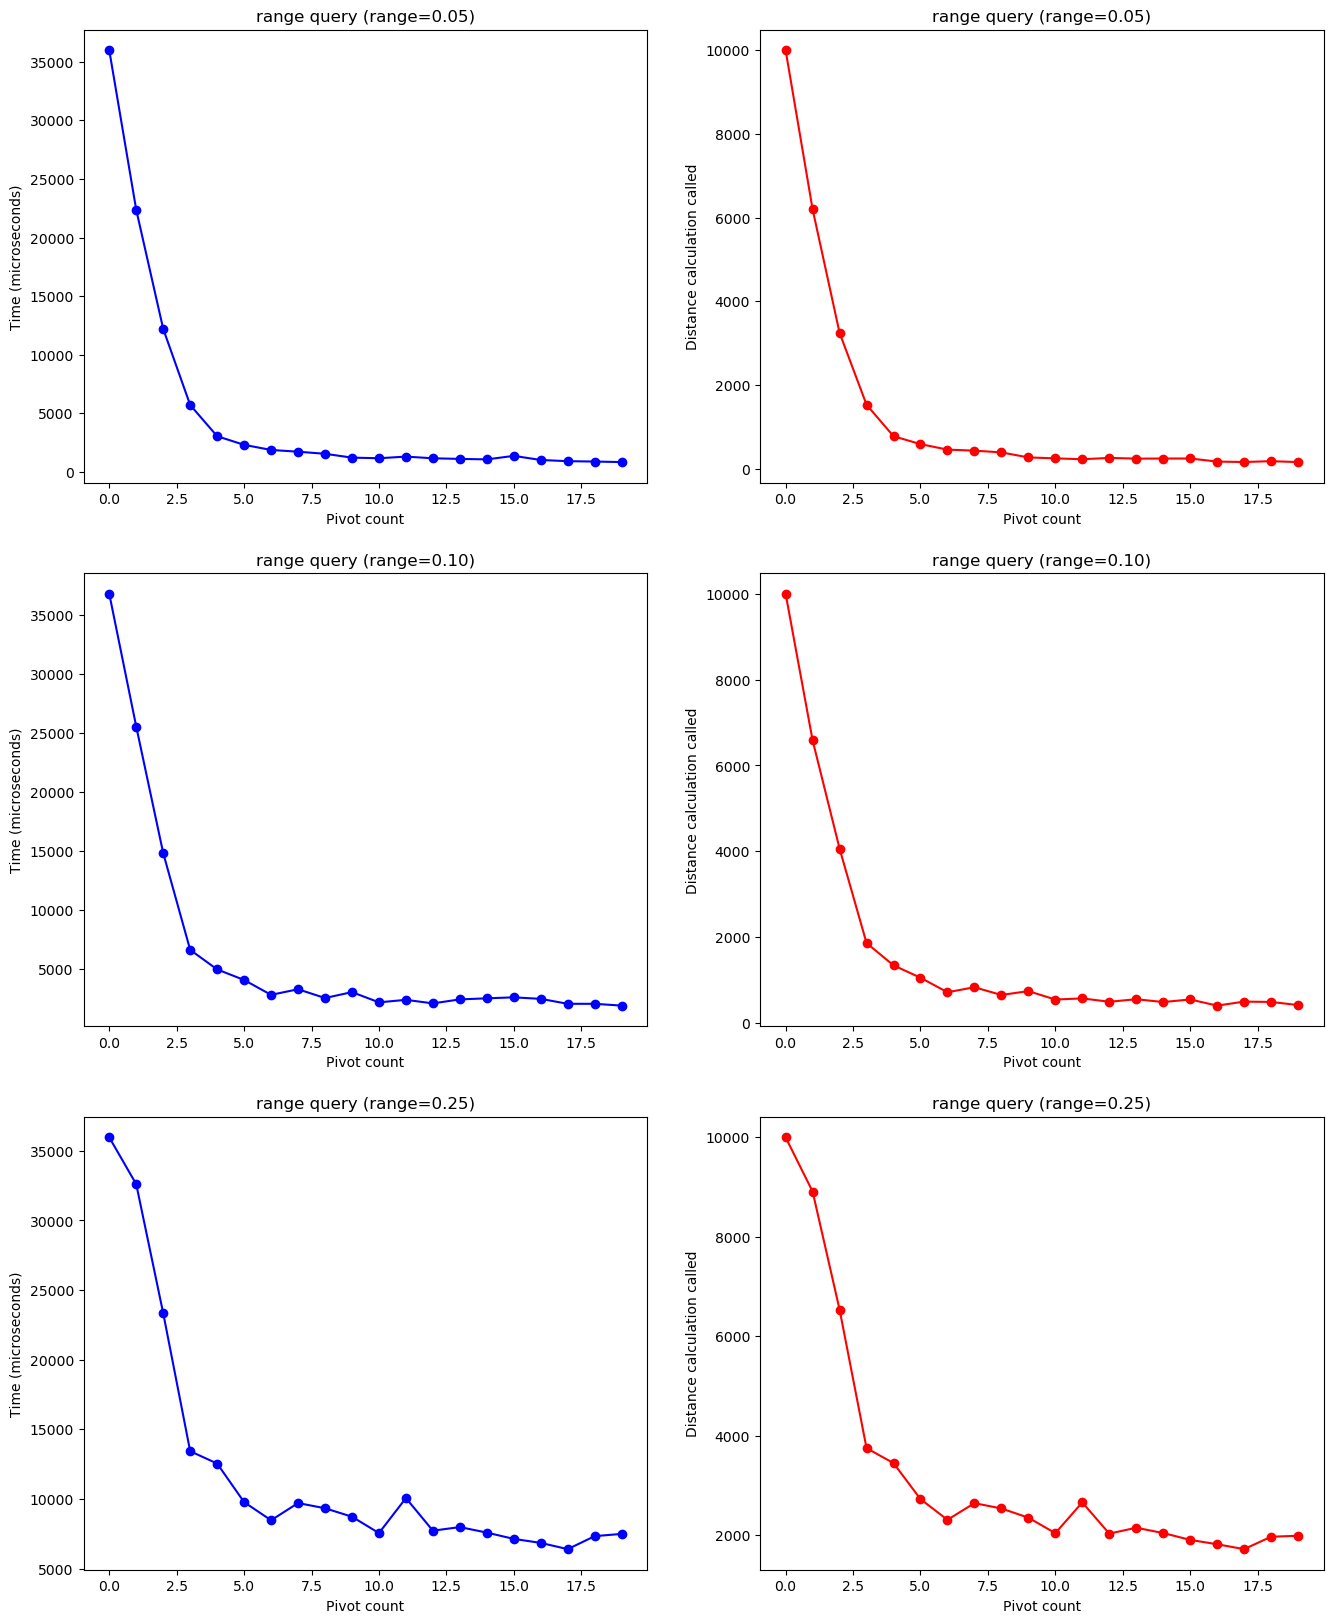
\includegraphics[width=\textwidth]{img/pivot_count_range.png}
    \caption{Rychlost a počet volání vzdálenostní funkce v závislosti na počtu pivotů (rozsahové dotazy)}
\end{figure}

\begin{figure}[H]
    \centering
    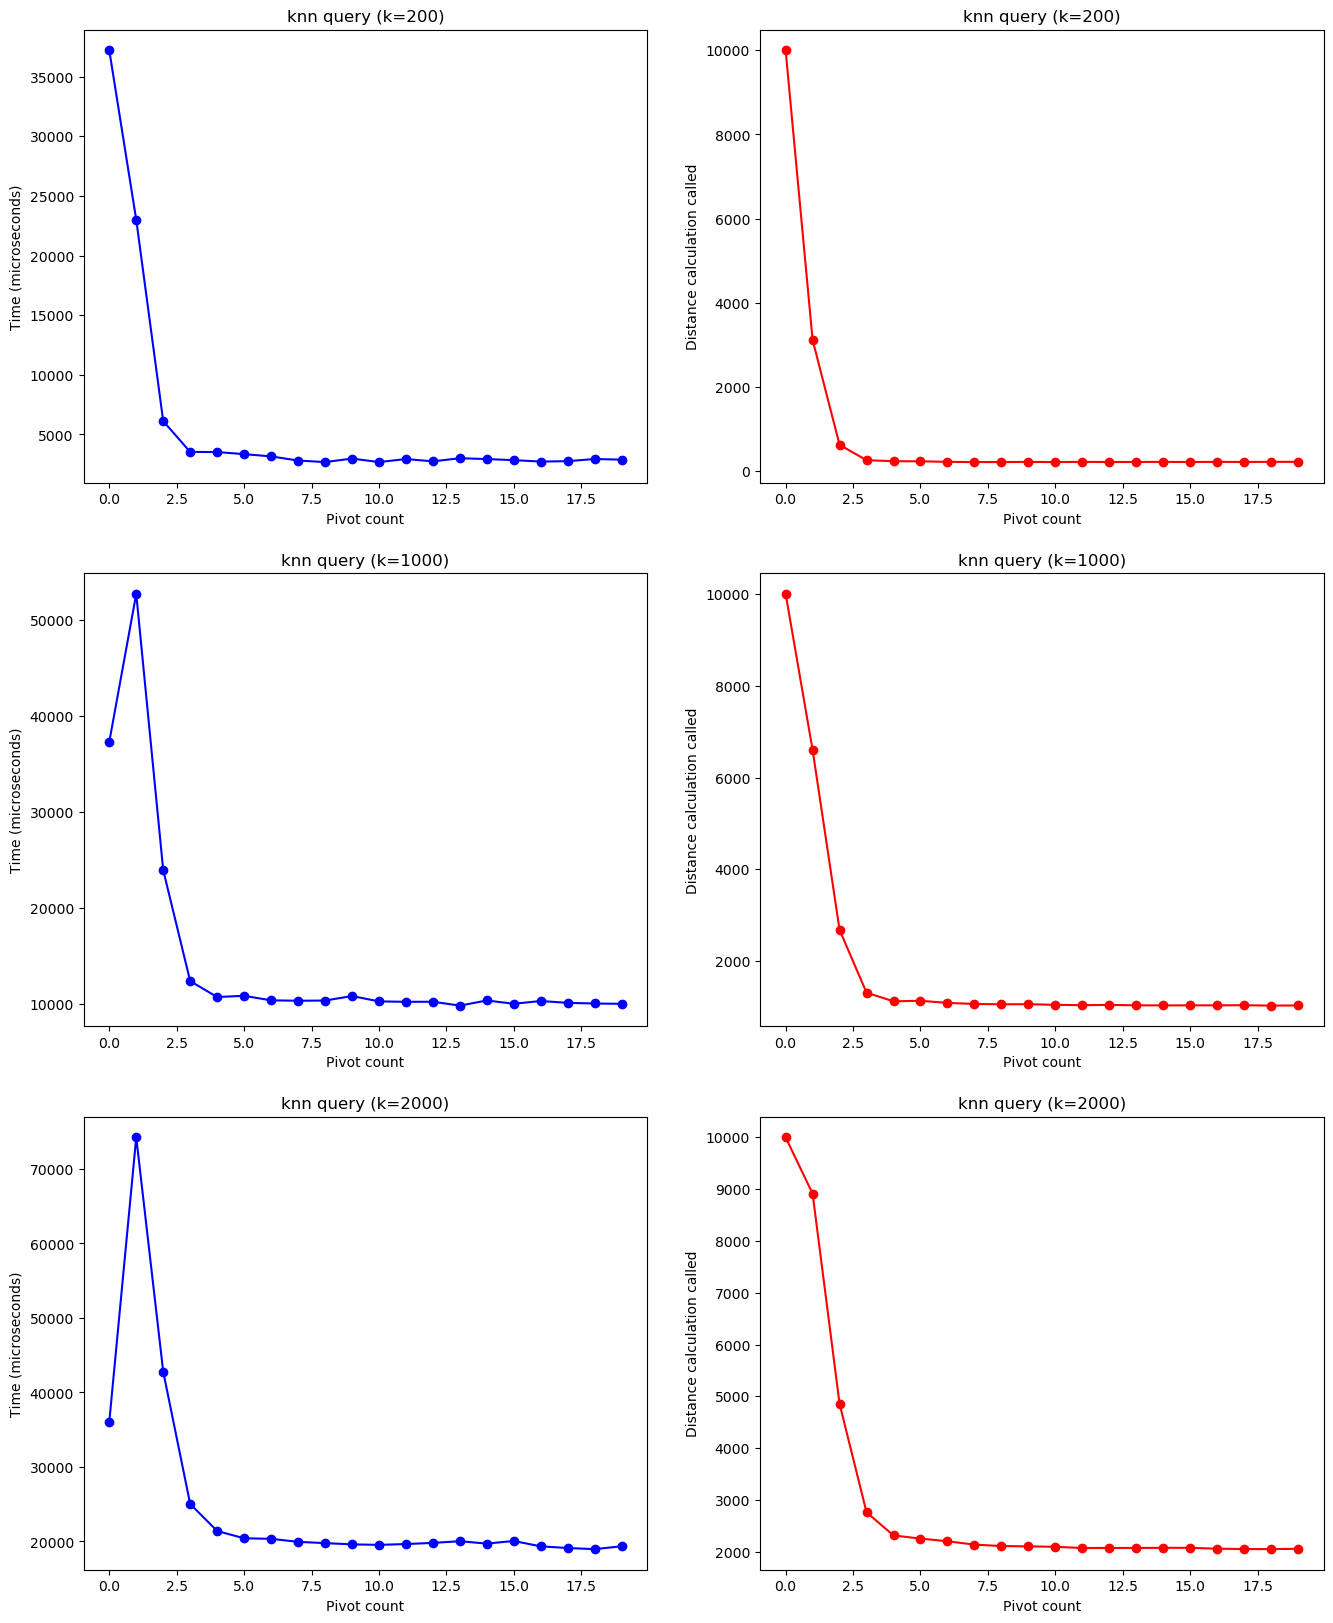
\includegraphics[width=\textwidth]{img/pivot_count_knn.png}
    \caption{Rychlost a počet volání vzdálenostní funkce v závislosti na počtu pivotů (knn dotazy)}
\end{figure}

\subsection{Porovnání rychlosti sekvenčního průchodu vs. indexu}

Porovnání rychlosti dotazů při použití indexu nebo sekvenčního průchodu ukazuje, že při použití indexu je možné dotazy zodpovědět za zlomek času. V tomto testu jsem měnil pouze velikost databáze (osa $x$), ostatní parametry indexu jsem neměnil. Čas sekvenčního průchodu roste lineárně s velikostí databáze. Čas při použití indexu se v případě některých dotazů chová téměř konstantně, v ostatních případech také roste lineárně, ale řádově pomaleji než při sekvenčním průchodu.

\begin{figure}[H]
    \centering
    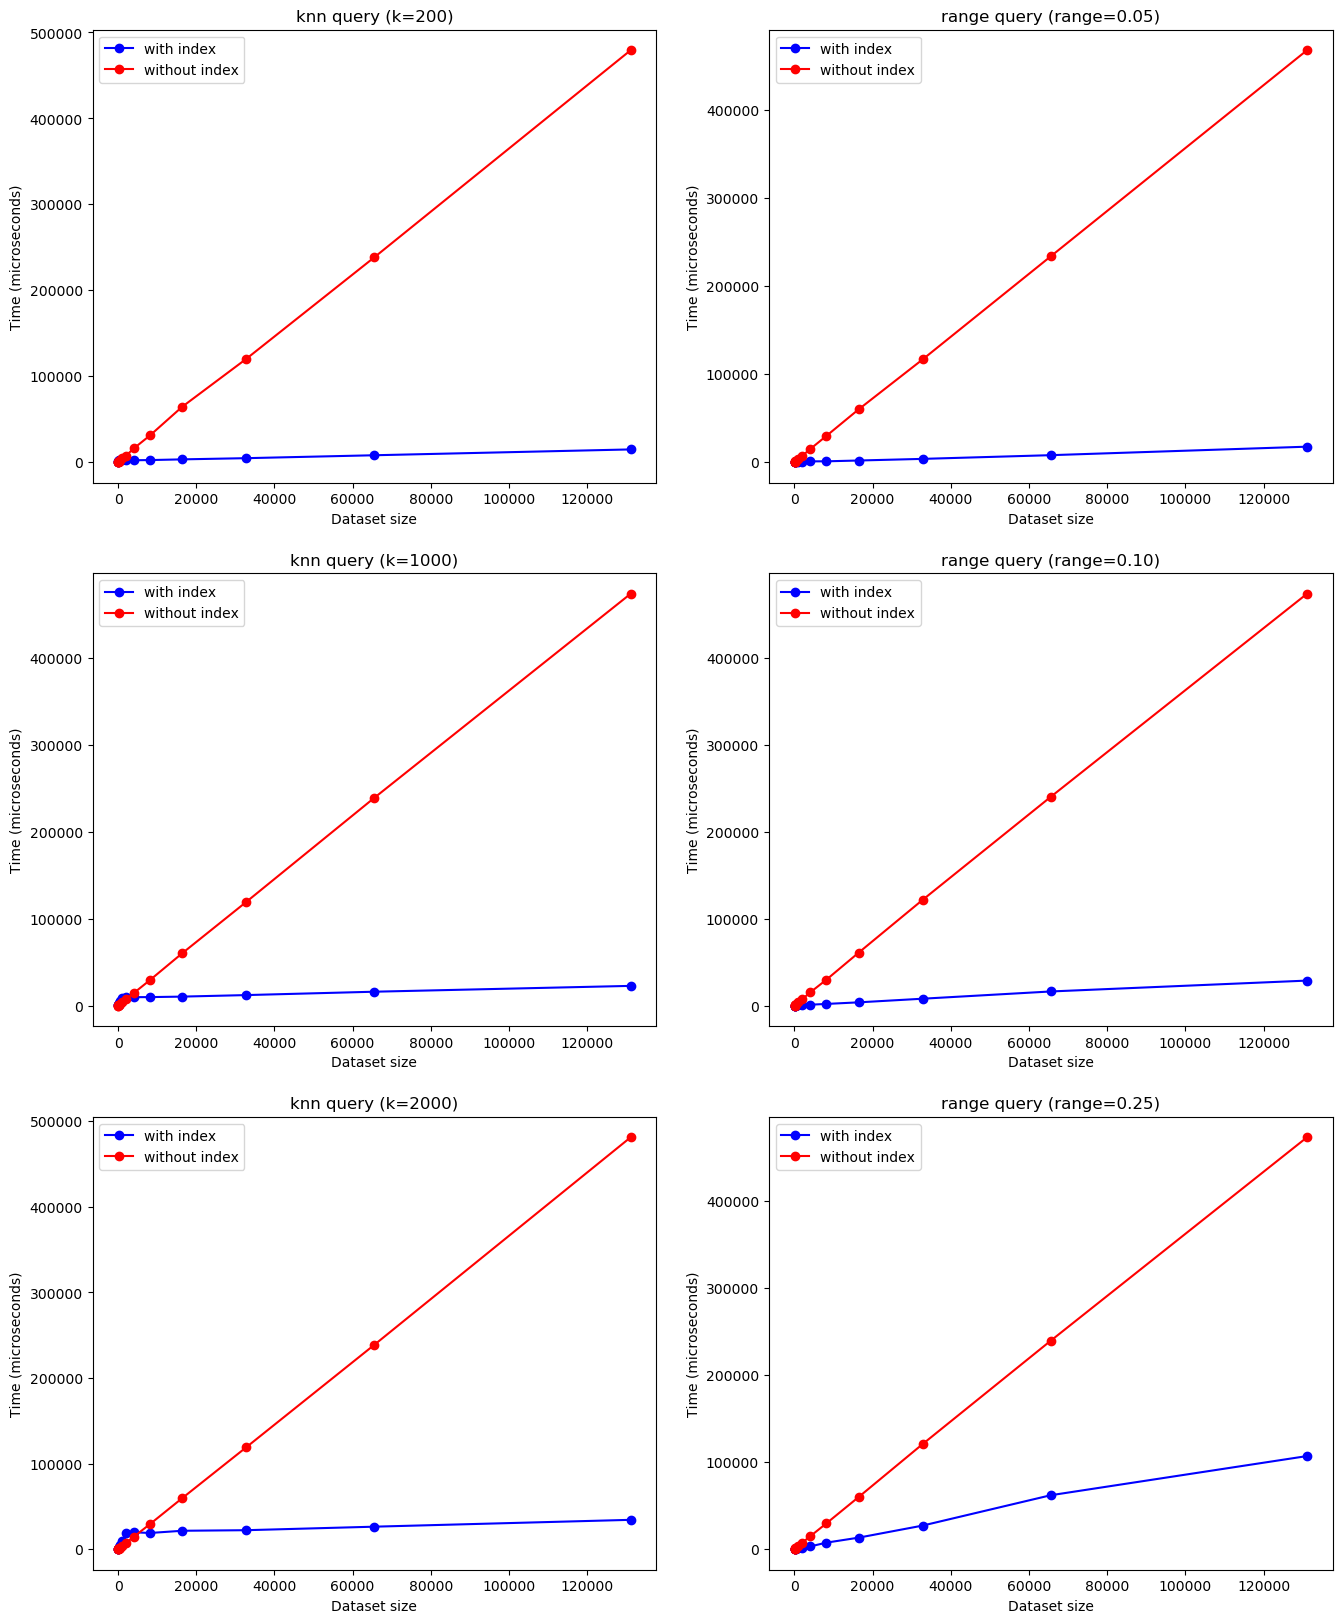
\includegraphics[width=0.9\textwidth]{with_index-without_index.png}
    \caption{Rychlost dotazů sekvenční průchod vs. index}
\end{figure}

\subsection{Vliv velikosti dimenze}

V posledním pokusu jsem se porovnával náročnost stejného dotazu na stejném množství dat, ale v různých dimenzích. Ve vyšších dimenzích se data od sebe vzdalují (prokletí dimenzionality), což vede k tomu, že se ve vyšších dimenzích nepodaří pomocí dolní meze odfiltrovat tolik bodů jako v nižších dimenzích. V tomto testu jsem měnil pouze dimenzi dat (osa $x$). Podle předpokladu došlo se zvyšující se dimenzí ke zhoršení jak času, tak i zvýšení počtu volání vzdálenostní funkce. Rychlost tohoto zvyšování zpomaluje se zvyšující se dimenzí. Počet volání vzdálenostní funkce nemůže překročit počet prvků v databázi.

\begin{figure}[H]
    \centering
    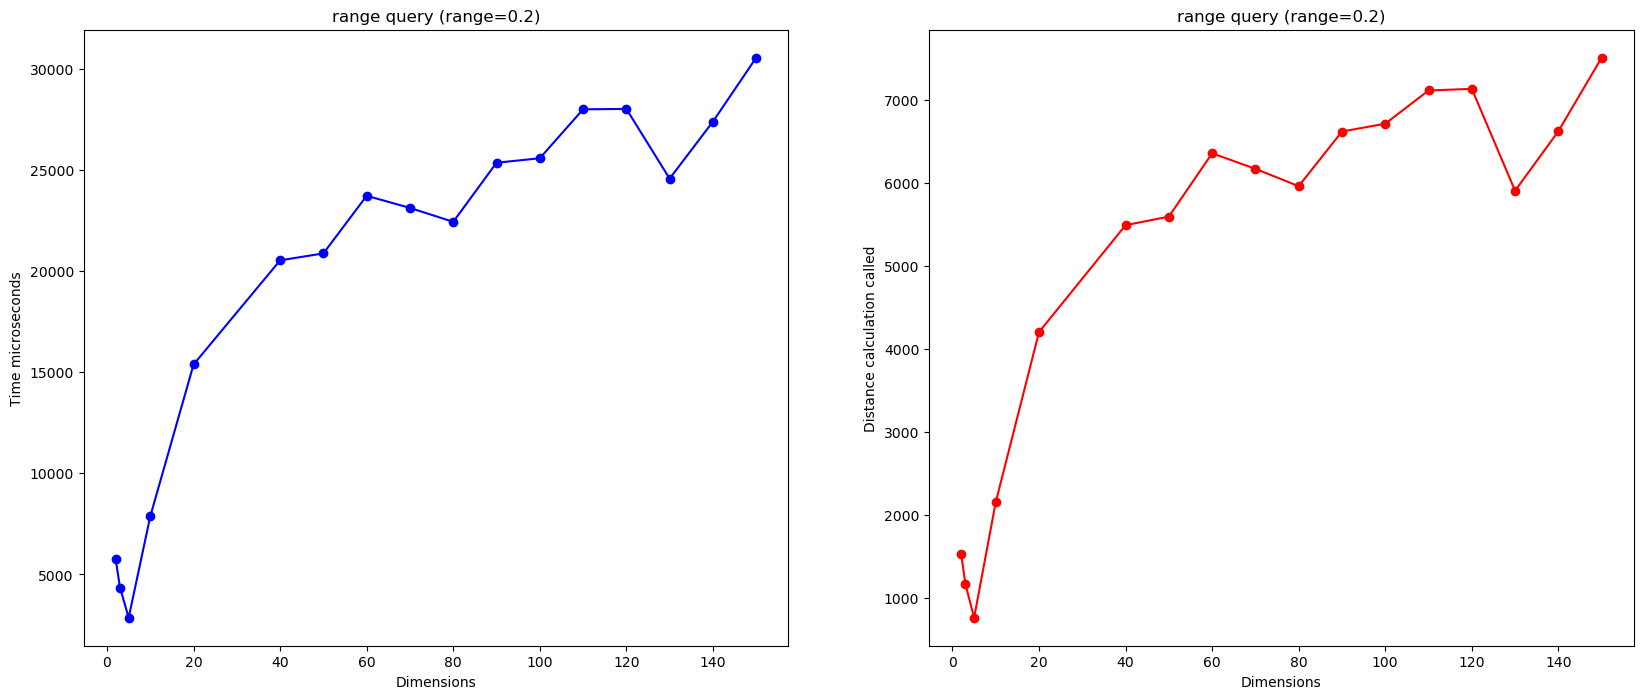
\includegraphics[width=0.9\textwidth]{dimensions.png}
    \caption{Rychlost a počet volání vzdálenostní funkce v závislosti na dimenzi dat}
\end{figure}

\section{Diskuze}

Vytvořená implementace je funkční, což ukazuje shoda výsledků sekvenčního průchodu a výsledků získaných za pomoci indexu. Nezaměřoval jsem se na ošetření mezních situací, jelikož podstatou tohoto projektu bylo vytvoření funkčního prototypu, zatímco řešit mezní situace by projekt znatelně zkomplikovalo, aniž by byl vidět jakýkoliv rozdíl v prováděných experimentech. 

Těžiště projektu spočívalo v implementaci LAESA a Jupyter notebooku, který obsahuje experimentální část. Projekt by bylo možné dále vylepšit doplněním webového rozhraní tak, aby podporovalo veškeré operace implementace LAESA (čtení/zápis do souboru, grafické zobrazení výsledku).

V případě, že by se mělo jednat o implementaci použitelnou v praxi, bylo by vhodnější použít nějaký rychlejší jazyk (např. C/C++) než Python, pro který jsem se rozhodl kvůli matematickým a grafickým knihovnám, které kód výrazně zjednodušily a zkrátily.

\section{Závěr}

V rámci zpracování projektu jsem si vyzkoušel implementovat jeden z možných způsobů indexace v $n$-dimenzionálním prostoru. Zaujalo mě, že využití tak jednoduchého konceptu jako je trojúhelníková nerovnost, může vést k tak výraznému zlepšení. Experimenty ukázaly, že dobrý počet pivotů se pohybuje okolo deseti. To je méně, než jsem očekával před provedením experimentální části. Dále se také ukázalo, že dosažené zrychlení je při porovnání se sekvenčním průchodem významné.

\end{document}

